\documentclass[11pt, oneside]{article} 	% use "amsart" instead of "article" for AMSLaTeX format
\usepackage{geometry} 		% See geometry.pdf to learn the layout options. There are lots.
\geometry{letterpaper}  		% ... or a4paper or a5paper or ... 
\usepackage[parfill]{parskip} 		% Activate to begin paragraphs with an empty line rather than an indent
\usepackage{graphicx}				% Use pdf, png, jpg, or eps§ with pdflatex; use eps in DVI mode
								% TeX will automatically convert eps --> pdf in pdflatex		
\usepackage{amssymb}
\usepackage{amsmath}
\usepackage{authblk}
\usepackage[
backend=biber,
style=alphabetic,
]{biblatex}
\usepackage{graphicx}
\graphicspath{ {./images/} }
\usepackage{verbatim}
\usepackage{tikz} 
\usepackage{subfig}
\usepackage{hyperref}

\usepackage{syntonly}
% \syntaxonly <-- use this for checking syntax only
% \mbox {text} - keep together
% \fbox {text} - keep together and draw around

%\pagestyle{plain|headings|empty} % header and footer p.27
%SetFonts
%\include{filename}, \includeonly{filename1, filename2} , \input[fiename}

%SetFonts% 

\title{The Office DVD Problem}
\author{Dave Fetterman}
\affil{Obviously Unemployed}
\date{7/13/22}
\begin{document}
\maketitle

Screensavers have captivated [this] man since the 1990s. If watched long enough, what will the spirits of the machine tell us?

Specifically, the question of whether a bouncing rectangle will slide \emph{exactly} into the corner of the screen, for a satisfying, perfectly diametric rebound, was even addressed on \emph{The Office}
\href{https://www.youtube.com/watch?v=QOtuX0jL85Y}{(link)}.

However, though these characters reportedly watched this sleep-mode drama play out for years until payoff, we ask - under what conditions will the rectangle \emph{definitely} perfectly bounce into the screen's corner?
 
\begin{figure}
\centering
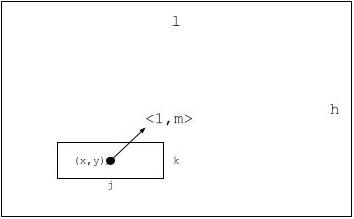
\includegraphics[scale=.5]{setup}
\caption{The Office DVD problem's most generic setup}
\end{figure}


\begin{figure}[!htb]
\centering
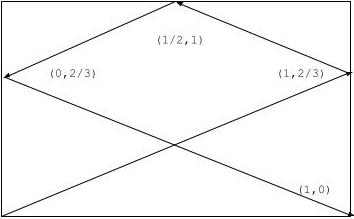
\includegraphics[scale=.5]{problem1trajectory}
 \caption{Success for $m = \frac{2}{3}, j, k = 0, h, l = 1$ (not to scale)}
\end{figure}

\subsection{Statement} 
Suppose we have a continuous screen of length $l$, height $h$, containing an axis-aligned rectangle of length $j$ and height $k$ centered at point $(x, y)$.

Suppose this rectangle is launched at direction $\langle 1, m\rangle$ \footnote {Think of this as slope $m$} and ``bounces'' according to billiard rules \footnote{Glancing off a top/bottom boundary, our trajectory goes from $\langle 1, m \rangle$ to $\langle 1, -m \rangle$, with $\langle \pm 1, m \rangle$ to $\langle \mp 1, m \rangle$ for a left/right one}.

Given $l, h, j, k, m \in \mathbb{R}$, can we tell whether the rectangle ever bounce perfectly into a corner?  

We can approach this problem from the simplest version to the most complex.

\subsection{Problem 1} 

Suppose $j = k = 0$ and $x = y = 0$. In other words, suppose we have a \emph{point} starting at the bottom left corner
 (origin). Under what conditions (i.e. choice of $m$) does this bounce into a corner?


\subsection{Problem 2} 

Suppose $j, k > 0, x = \frac{j}{2}, y = \frac{k}{2}$. In other words, suppose we have a rectangle starting at the bottom left corner. Under what conditions does this bounce into a corner?

\subsection{Problem 3} 

Suppose we have maximally open (reasonable) conditions, with $x \in [\frac{j}{2}, l - \frac{j}{2}], y \in [\frac{k}{2}, h - \frac{k}{2}]$ (that is, a $j \times k$ rectangle fitting entirely in the screen). Under what conditions does this bounce into a corner?


\subsection{Problem 4} 

Some clowns \footnote {J. H. Wang, N. H. Talbert, L. F. Waldman} have come along demanding a version of the setup respecting the discrete (pixellated) nature of digital screens.  Very well.

For each of problem 1, 2, and 3, how does the answer change if the screen comprises square pixels of length \footnote{If $p$ is not a whole number, this can be normalized} $p \in \mathbb{N}$ , where $p | j, k, h, l$, and ``meeting a corner" means a corner of the small (continuous) rectangle meets a wall within length $p$ of the corner point?








\end{document}
